\section{Task 1 --- Conceptual Modelling and Relational Design}

\subsection{Proximity definition}
We define proximity between HDB buildings and hawker centres using their coordinates.
The Haversine formula gives great-circle distance; we multiply by $1.5$ to estimate walking distance along roads and footpaths.
This approximation avoids routing each building--centre pair through an external service and can be reproduced offline.

Estimated walking distance is classified into three half-open intervals stored in \texttt{proximity\_level} (Table~\ref{tab:levels}).
Pairs at $2{,}400\,\mathrm{m}$ or more are not stored.
Transactions for buildings with no centre within range remain in the database but are excluded from Q4--Q6.
With the 2017-onwards file alone, 3{,}991 buildings have their nearest centre in level~1, 3{,}638 in level~2, 1{,}499 in level~3, and 625 have none within range (quality report for \texttt{step\_1}).

\begin{table}[H]
\centering
\caption{Proximity levels as half-open intervals of estimated walking distance.}
\label{tab:levels}
\begin{tabular}{@{}cll@{}}
\toprule
Level & Label & Walking distance \\
\midrule
1 & Walking distance & $[0, 800)$ m \\
2 & Nearby & $[800, 1{,}600)$ m \\
3 & Accessible & $[1{,}600, 2{,}400)$ m \\
\bottomrule
\end{tabular}
\end{table}

\subsection{Entity--relationship diagram}
Figure~\ref{fig:er} shows the revised Chen-style ER diagram with keys and $(\mathrm{min},\mathrm{max})$ cardinalities.
Town, HDBBuilding, HDBFlat and ResaleTransaction form a chain of one-to-many relationships.
The source files contain no unit number, so HDBFlat represents a \emph{flat profile} defined by type, model, floor area, storey range and lease commence year.
Several physical flats can share a profile.
Proximity is a many-to-many relationship between buildings and hawker centres with attribute \texttt{distance\_m}.
The proximity level of a pair is determined by distance, so ClassifiedAs is a derived (dashed) association via the level intervals rather than a stored attribute on Proximity.

\begin{landscape}
\begin{figure}[p]
\centering
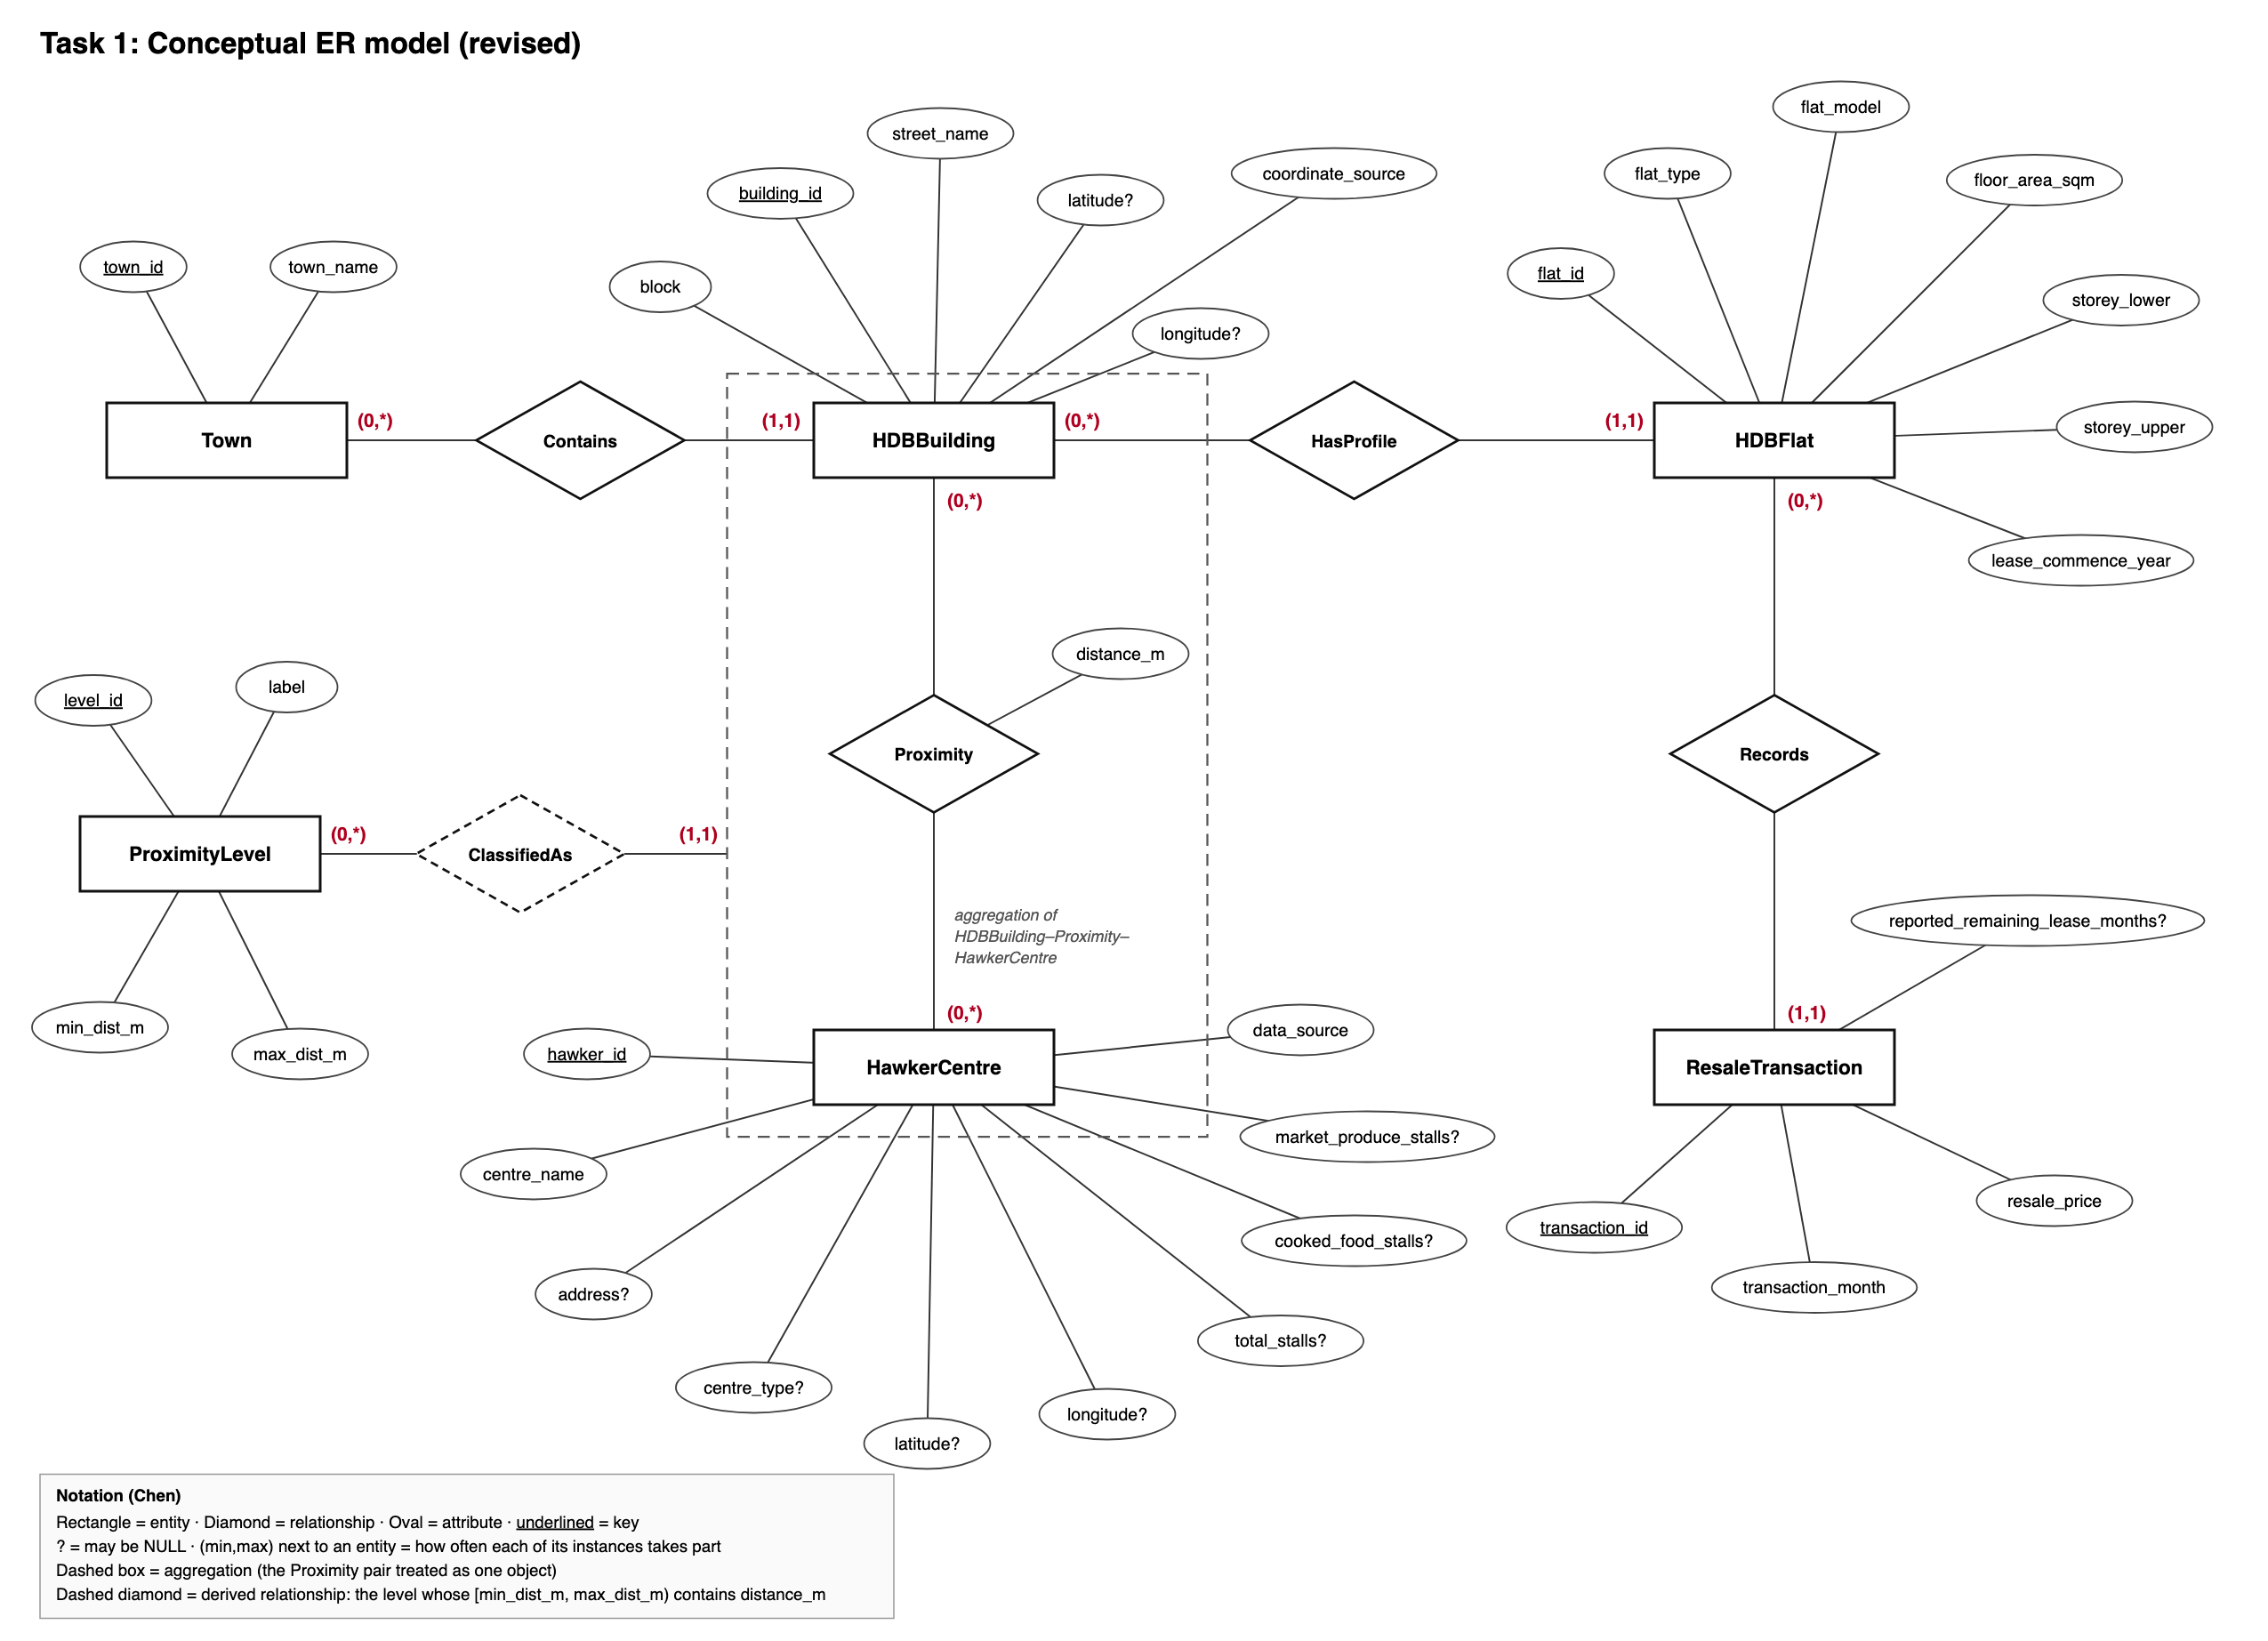
\includegraphics[width=0.95\linewidth,height=0.82\textheight,keepaspectratio]{figures/er_diagram.png}
\caption{Complete ER diagram for the revised design (keys and $(\mathrm{min},\mathrm{max})$ cardinalities).}
\label{fig:er}
\end{figure}
\end{landscape}

\subsection{Logical schema and data dictionary}
One-to-many relationships become foreign keys.
Proximity becomes table \texttt{proximity} keyed by $(\texttt{building\_id},\texttt{hawker\_id})$.
We derive the proximity level from the distance intervals to avoid storing the same classification twice.
Queries obtain the level by joining \texttt{proximity\_level} on $\texttt{min\_dist\_m} \le \texttt{distance\_m} < \texttt{max\_dist\_m}$.
We also store just one distance measure, since estimated walking distance is a fixed multiple of straight-line distance.

Table~\ref{tab:dict} summarises the seven relations.
The full \texttt{CREATE TABLE} script is in Appendix~\ref{app:schema} (\texttt{sql/schema.sql}).

\begin{table}[H]
\centering
\caption{Seven-table data dictionary (revised schema).}
\label{tab:dict}
\footnotesize
\begin{tabularx}{\textwidth}{@{}p{3.2cm}p{3.3cm}X@{}}
\toprule
Table & Primary key & Important attributes / constraints \\
\midrule
\texttt{town} & \texttt{town\_id} & Unique upper-case \texttt{town\_name}. \\
\texttt{hdb\_building} & \texttt{building\_id} & FK to town; unique $(\texttt{block},\texttt{street\_name})$; optional coordinates in Singapore bbox; \texttt{coordinate\_source}. \\
\texttt{hdb\_flat} & \texttt{flat\_id} & FK to building; unique flat profile; seven flat types; positive area; storey range; lease year 1960--2100. \\
\texttt{resale\_transaction} & \texttt{transaction\_id} & FK to flat; month on first of month $\ge$ 1990-01-01; positive price; optional reported remaining lease (months). \\
\texttt{hawker\_centre} & \texttt{hawker\_id} & Unique name; type HC/MHC/MK; stall counts; coordinates; data source tag. \\
\texttt{proximity\_level} & \texttt{level\_id} & Unique label; half-open distance interval; GiST exclusion prevents overlap. \\
\texttt{proximity} & \texttt{building\_id}, \texttt{hawker\_id} & FKs to building and hawker; non-negative \texttt{distance\_m}. \\
\bottomrule
\end{tabularx}
\end{table}

\paragraph{Why \texttt{lease\_commence\_year} stays on the flat.}
Across all five resale files, three buildings have two different lease commence years.
Keeping the year on the flat profile preserves these differences within a building.

\paragraph{Normalisation.}
We separate town names, building addresses, flat profiles and transactions so that each fact is stored at its appropriate level.
Town name, building address and the complete flat profile are declared unique alternate keys.
For proximity, the building--hawker pair determines distance, while the non-overlapping intervals determine its classification.
Under these modelled dependencies, each non-trivial determinant is a candidate key, giving a BCNF design.
The surrogate keys simplify joins, and the corresponding uniqueness constraints preserve the natural identifiers (Appendix~\ref{app:schema}).
No Task~4 performance indexes are created in the schema script---only the indexes PostgreSQL creates for PRIMARY KEY, UNIQUE and EXCLUDE.

\subsection{Implementation}
The schema is created in one transaction by \texttt{Task 1/revised/schema.sql} (copied to Appendix~\ref{app:schema}).
Bulk load uses server-side \texttt{COPY} from the seven CSVs of a chosen step (\texttt{load\_data.sql}).
Constraints reject invalid states at load time (canonical text, flat types, positive prices and areas, Singapore coordinate bounds, non-overlapping levels).
